\sujet{SUSAN corner detector}

\noindent
{\bf Duration: 1h30 / 20 points}

All documents allowed. NO internet connection, except for connection to campus website (to download the test images and to upload your results, and to use the different electronic documents).

\begin{wikipedia}
 
SUSAN is an acronym standing for ''smallest univalue segment assimilating nucleus.''  This method is the subject of a 1994 UK patent which is no longer in force.

For feature detection, SUSAN places a circular mask over the pixel to be tested (the nucleus). The region of the mask is $M$, and a pixel in this mask is represented by $\vec{m} \in M$. The nucleus is at $\vec{m}_0$. Every pixel is compared to the nucleus using the comparison function:

$$
c(\vec{m}) = e^{-\left(\frac{I(\vec{m}) - I(\vec{m}_0)}{t}\right)^6}
$$

where $t$ is the brightness difference threshold $I$ is the brightness of the pixel and the power of the exponent has been determined empirically. This function has the appearance of a smoothed top-hat or rectangular function. The area of the SUSAN is given by:

$$
n(M) = \sum_{\vec{m}\in M} c(\vec{m})
$$

If $c$ is the rectangular function, then $n$ is the number of pixels in the mask which are within $t$ of the nucleus. The response of the SUSAN operator is given by:

$$
R(M) =     \begin{array}{ll}
               g - n(M) & \mbox{if}\ n(M) < g\\
               0        & \mbox{otherwise,}
           \end{array}
$$

where $g$ is named the `geometric threshold'. In other words, the SUSAN operator only has a positive score if the area is small enough. The smallest SUSAN locally can be found using non-maximal suppression, and this is the complete SUSAN operator.

The value $t$ determines how similar points have to be to the nucleus before they are considered to be part of the univalue segment. The value of $g$ determines the minimum size of the univalue segment. If $g$ is large enough, then this becomes an edge detection.

For corner detection, two further steps are used. Firstly, the centroid of the SUSAN is found. A proper corner will have the centroid far from the nucleus. The second step insists that all points on the line from the nucleus through the centroid out to the edge of the mask are in the SUSAN.

\end{wikipedia}

\section{Comparison function(6 points)} 
\begin{qbox}
Code a function that computes $c$ for a given region size $W$.

\end{qbox}\begin{matlab}
function c = comparisonFunction(I, W, t)
\end{matlab}

\section{Area (4 points)}
\begin{qbox}
Code a functions that evaluates the area of the SUSAN.

\end{qbox}\begin{matlab}
function n = susanArea(c)
\end{matlab}

\section{Response (10 points)}
\begin{qbox}

\begin{itemize}
 \item[4 pts]
Code the response function

\item [4 pts]
Perform the last steps for corner detection, and apply on two images of Fig.\ref{fig:exam:2018:retake:ipr:examples}. 
\item [2 pts] Test different values of $g$ and  $t$ (justify your choices). Illustrate the edge detection.
\end{itemize}



\end{qbox}\begin{matlab}
function R = response(n, g)
\end{matlab}

\begin{figure}
 \centering
 \subfloat[Wild roar image.]{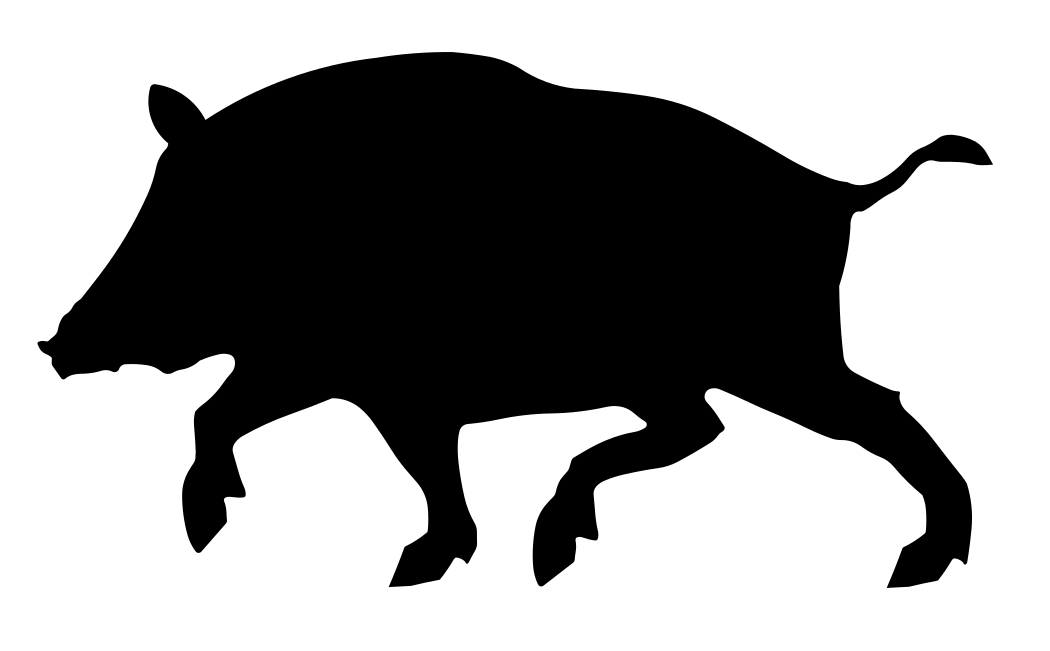
\includegraphics[width=.45\linewidth]{sweden_road.png}}
 \hfill
 \subfloat[Square image.]{
\includegraphics[width=.3\linewidth]{square.png}}
 \caption{Application examples.}
 \label{fig:exam:2018:retake:ipr:examples}
\end{figure}

